\documentclass[11pt]{article}

    \usepackage[breakable]{tcolorbox}
    \usepackage{parskip} % Stop auto-indenting (to mimic markdown behaviour)
    

    % Basic figure setup, for now with no caption control since it's done
    % automatically by Pandoc (which extracts ![](path) syntax from Markdown).
    \usepackage{graphicx}
    % Maintain compatibility with old templates. Remove in nbconvert 6.0
    \let\Oldincludegraphics\includegraphics
    % Ensure that by default, figures have no caption (until we provide a
    % proper Figure object with a Caption API and a way to capture that
    % in the conversion process - todo).
    \usepackage{caption}
    \DeclareCaptionFormat{nocaption}{}
    \captionsetup{format=nocaption,aboveskip=0pt,belowskip=0pt}

    \usepackage{float}
    \floatplacement{figure}{H} % forces figures to be placed at the correct location
    \usepackage{xcolor} % Allow colors to be defined
    \usepackage{enumerate} % Needed for markdown enumerations to work
    \usepackage{geometry} % Used to adjust the document margins
    \usepackage{amsmath} % Equations
    \usepackage{amssymb} % Equations
    \usepackage{textcomp} % defines textquotesingle
    % Hack from http://tex.stackexchange.com/a/47451/13684:
    \AtBeginDocument{%
        \def\PYZsq{\textquotesingle}% Upright quotes in Pygmentized code
    }
    \usepackage{upquote} % Upright quotes for verbatim code
    \usepackage{eurosym} % defines \euro

    \usepackage{iftex}
    \ifPDFTeX
        \usepackage[T1]{fontenc}
        \IfFileExists{alphabeta.sty}{
              \usepackage{alphabeta}
          }{
              \usepackage[mathletters]{ucs}
              \usepackage[utf8x]{inputenc}
          }
    \else
        \usepackage{fontspec}
        \usepackage{unicode-math}
    \fi

    \usepackage{fancyvrb} % verbatim replacement that allows latex
    \usepackage{grffile} % extends the file name processing of package graphics
                         % to support a larger range
    \makeatletter % fix for old versions of grffile with XeLaTeX
    \@ifpackagelater{grffile}{2019/11/01}
    {
      % Do nothing on new versions
    }
    {
      \def\Gread@@xetex#1{%
        \IfFileExists{"\Gin@base".bb}%
        {\Gread@eps{\Gin@base.bb}}%
        {\Gread@@xetex@aux#1}%
      }
    }
    \makeatother
    \usepackage[Export]{adjustbox} % Used to constrain images to a maximum size
    \adjustboxset{max size={0.9\linewidth}{0.9\paperheight}}

    % The hyperref package gives us a pdf with properly built
    % internal navigation ('pdf bookmarks' for the table of contents,
    % internal cross-reference links, web links for URLs, etc.)
    \usepackage{hyperref}
    % The default LaTeX title has an obnoxious amount of whitespace. By default,
    % titling removes some of it. It also provides customization options.
    \usepackage{titling}
    \usepackage{longtable} % longtable support required by pandoc >1.10
    \usepackage{booktabs}  % table support for pandoc > 1.12.2
    \usepackage{array}     % table support for pandoc >= 2.11.3
    \usepackage{calc}      % table minipage width calculation for pandoc >= 2.11.1
    \usepackage[inline]{enumitem} % IRkernel/repr support (it uses the enumerate* environment)
    \usepackage[normalem]{ulem} % ulem is needed to support strikethroughs (\sout)
                                % normalem makes italics be italics, not underlines
    \usepackage{mathrsfs}
    

    
    % Colors for the hyperref package
    \definecolor{urlcolor}{rgb}{0,.145,.698}
    \definecolor{linkcolor}{rgb}{.71,0.21,0.01}
    \definecolor{citecolor}{rgb}{.12,.54,.11}

    % ANSI colors
    \definecolor{ansi-black}{HTML}{3E424D}
    \definecolor{ansi-black-intense}{HTML}{282C36}
    \definecolor{ansi-red}{HTML}{E75C58}
    \definecolor{ansi-red-intense}{HTML}{B22B31}
    \definecolor{ansi-green}{HTML}{00A250}
    \definecolor{ansi-green-intense}{HTML}{007427}
    \definecolor{ansi-yellow}{HTML}{DDB62B}
    \definecolor{ansi-yellow-intense}{HTML}{B27D12}
    \definecolor{ansi-blue}{HTML}{208FFB}
    \definecolor{ansi-blue-intense}{HTML}{0065CA}
    \definecolor{ansi-magenta}{HTML}{D160C4}
    \definecolor{ansi-magenta-intense}{HTML}{A03196}
    \definecolor{ansi-cyan}{HTML}{60C6C8}
    \definecolor{ansi-cyan-intense}{HTML}{258F8F}
    \definecolor{ansi-white}{HTML}{C5C1B4}
    \definecolor{ansi-white-intense}{HTML}{A1A6B2}
    \definecolor{ansi-default-inverse-fg}{HTML}{FFFFFF}
    \definecolor{ansi-default-inverse-bg}{HTML}{000000}

    % common color for the border for error outputs.
    \definecolor{outerrorbackground}{HTML}{FFDFDF}

    % commands and environments needed by pandoc snippets
    % extracted from the output of `pandoc -s`
    \providecommand{\tightlist}{%
      \setlength{\itemsep}{0pt}\setlength{\parskip}{0pt}}
    \DefineVerbatimEnvironment{Highlighting}{Verbatim}{commandchars=\\\{\}}
    % Add ',fontsize=\small' for more characters per line
    \newenvironment{Shaded}{}{}
    \newcommand{\KeywordTok}[1]{\textcolor[rgb]{0.00,0.44,0.13}{\textbf{{#1}}}}
    \newcommand{\DataTypeTok}[1]{\textcolor[rgb]{0.56,0.13,0.00}{{#1}}}
    \newcommand{\DecValTok}[1]{\textcolor[rgb]{0.25,0.63,0.44}{{#1}}}
    \newcommand{\BaseNTok}[1]{\textcolor[rgb]{0.25,0.63,0.44}{{#1}}}
    \newcommand{\FloatTok}[1]{\textcolor[rgb]{0.25,0.63,0.44}{{#1}}}
    \newcommand{\CharTok}[1]{\textcolor[rgb]{0.25,0.44,0.63}{{#1}}}
    \newcommand{\StringTok}[1]{\textcolor[rgb]{0.25,0.44,0.63}{{#1}}}
    \newcommand{\CommentTok}[1]{\textcolor[rgb]{0.38,0.63,0.69}{\textit{{#1}}}}
    \newcommand{\OtherTok}[1]{\textcolor[rgb]{0.00,0.44,0.13}{{#1}}}
    \newcommand{\AlertTok}[1]{\textcolor[rgb]{1.00,0.00,0.00}{\textbf{{#1}}}}
    \newcommand{\FunctionTok}[1]{\textcolor[rgb]{0.02,0.16,0.49}{{#1}}}
    \newcommand{\RegionMarkerTok}[1]{{#1}}
    \newcommand{\ErrorTok}[1]{\textcolor[rgb]{1.00,0.00,0.00}{\textbf{{#1}}}}
    \newcommand{\NormalTok}[1]{{#1}}

    % Additional commands for more recent versions of Pandoc
    \newcommand{\ConstantTok}[1]{\textcolor[rgb]{0.53,0.00,0.00}{{#1}}}
    \newcommand{\SpecialCharTok}[1]{\textcolor[rgb]{0.25,0.44,0.63}{{#1}}}
    \newcommand{\VerbatimStringTok}[1]{\textcolor[rgb]{0.25,0.44,0.63}{{#1}}}
    \newcommand{\SpecialStringTok}[1]{\textcolor[rgb]{0.73,0.40,0.53}{{#1}}}
    \newcommand{\ImportTok}[1]{{#1}}
    \newcommand{\DocumentationTok}[1]{\textcolor[rgb]{0.73,0.13,0.13}{\textit{{#1}}}}
    \newcommand{\AnnotationTok}[1]{\textcolor[rgb]{0.38,0.63,0.69}{\textbf{\textit{{#1}}}}}
    \newcommand{\CommentVarTok}[1]{\textcolor[rgb]{0.38,0.63,0.69}{\textbf{\textit{{#1}}}}}
    \newcommand{\VariableTok}[1]{\textcolor[rgb]{0.10,0.09,0.49}{{#1}}}
    \newcommand{\ControlFlowTok}[1]{\textcolor[rgb]{0.00,0.44,0.13}{\textbf{{#1}}}}
    \newcommand{\OperatorTok}[1]{\textcolor[rgb]{0.40,0.40,0.40}{{#1}}}
    \newcommand{\BuiltInTok}[1]{{#1}}
    \newcommand{\ExtensionTok}[1]{{#1}}
    \newcommand{\PreprocessorTok}[1]{\textcolor[rgb]{0.74,0.48,0.00}{{#1}}}
    \newcommand{\AttributeTok}[1]{\textcolor[rgb]{0.49,0.56,0.16}{{#1}}}
    \newcommand{\InformationTok}[1]{\textcolor[rgb]{0.38,0.63,0.69}{\textbf{\textit{{#1}}}}}
    \newcommand{\WarningTok}[1]{\textcolor[rgb]{0.38,0.63,0.69}{\textbf{\textit{{#1}}}}}


    % Define a nice break command that doesn't care if a line doesn't already
    % exist.
    \def\br{\hspace*{\fill} \\* }
    % Math Jax compatibility definitions
    \def\gt{>}
    \def\lt{<}
    \let\Oldtex\TeX
    \let\Oldlatex\LaTeX
    \renewcommand{\TeX}{\textrm{\Oldtex}}
    \renewcommand{\LaTeX}{\textrm{\Oldlatex}}
    % Document parameters
    % Document title
    \title{report}
    
    
    
    
    
% Pygments definitions
\makeatletter
\def\PY@reset{\let\PY@it=\relax \let\PY@bf=\relax%
    \let\PY@ul=\relax \let\PY@tc=\relax%
    \let\PY@bc=\relax \let\PY@ff=\relax}
\def\PY@tok#1{\csname PY@tok@#1\endcsname}
\def\PY@toks#1+{\ifx\relax#1\empty\else%
    \PY@tok{#1}\expandafter\PY@toks\fi}
\def\PY@do#1{\PY@bc{\PY@tc{\PY@ul{%
    \PY@it{\PY@bf{\PY@ff{#1}}}}}}}
\def\PY#1#2{\PY@reset\PY@toks#1+\relax+\PY@do{#2}}

\@namedef{PY@tok@w}{\def\PY@tc##1{\textcolor[rgb]{0.73,0.73,0.73}{##1}}}
\@namedef{PY@tok@c}{\let\PY@it=\textit\def\PY@tc##1{\textcolor[rgb]{0.24,0.48,0.48}{##1}}}
\@namedef{PY@tok@cp}{\def\PY@tc##1{\textcolor[rgb]{0.61,0.40,0.00}{##1}}}
\@namedef{PY@tok@k}{\let\PY@bf=\textbf\def\PY@tc##1{\textcolor[rgb]{0.00,0.50,0.00}{##1}}}
\@namedef{PY@tok@kp}{\def\PY@tc##1{\textcolor[rgb]{0.00,0.50,0.00}{##1}}}
\@namedef{PY@tok@kt}{\def\PY@tc##1{\textcolor[rgb]{0.69,0.00,0.25}{##1}}}
\@namedef{PY@tok@o}{\def\PY@tc##1{\textcolor[rgb]{0.40,0.40,0.40}{##1}}}
\@namedef{PY@tok@ow}{\let\PY@bf=\textbf\def\PY@tc##1{\textcolor[rgb]{0.67,0.13,1.00}{##1}}}
\@namedef{PY@tok@nb}{\def\PY@tc##1{\textcolor[rgb]{0.00,0.50,0.00}{##1}}}
\@namedef{PY@tok@nf}{\def\PY@tc##1{\textcolor[rgb]{0.00,0.00,1.00}{##1}}}
\@namedef{PY@tok@nc}{\let\PY@bf=\textbf\def\PY@tc##1{\textcolor[rgb]{0.00,0.00,1.00}{##1}}}
\@namedef{PY@tok@nn}{\let\PY@bf=\textbf\def\PY@tc##1{\textcolor[rgb]{0.00,0.00,1.00}{##1}}}
\@namedef{PY@tok@ne}{\let\PY@bf=\textbf\def\PY@tc##1{\textcolor[rgb]{0.80,0.25,0.22}{##1}}}
\@namedef{PY@tok@nv}{\def\PY@tc##1{\textcolor[rgb]{0.10,0.09,0.49}{##1}}}
\@namedef{PY@tok@no}{\def\PY@tc##1{\textcolor[rgb]{0.53,0.00,0.00}{##1}}}
\@namedef{PY@tok@nl}{\def\PY@tc##1{\textcolor[rgb]{0.46,0.46,0.00}{##1}}}
\@namedef{PY@tok@ni}{\let\PY@bf=\textbf\def\PY@tc##1{\textcolor[rgb]{0.44,0.44,0.44}{##1}}}
\@namedef{PY@tok@na}{\def\PY@tc##1{\textcolor[rgb]{0.41,0.47,0.13}{##1}}}
\@namedef{PY@tok@nt}{\let\PY@bf=\textbf\def\PY@tc##1{\textcolor[rgb]{0.00,0.50,0.00}{##1}}}
\@namedef{PY@tok@nd}{\def\PY@tc##1{\textcolor[rgb]{0.67,0.13,1.00}{##1}}}
\@namedef{PY@tok@s}{\def\PY@tc##1{\textcolor[rgb]{0.73,0.13,0.13}{##1}}}
\@namedef{PY@tok@sd}{\let\PY@it=\textit\def\PY@tc##1{\textcolor[rgb]{0.73,0.13,0.13}{##1}}}
\@namedef{PY@tok@si}{\let\PY@bf=\textbf\def\PY@tc##1{\textcolor[rgb]{0.64,0.35,0.47}{##1}}}
\@namedef{PY@tok@se}{\let\PY@bf=\textbf\def\PY@tc##1{\textcolor[rgb]{0.67,0.36,0.12}{##1}}}
\@namedef{PY@tok@sr}{\def\PY@tc##1{\textcolor[rgb]{0.64,0.35,0.47}{##1}}}
\@namedef{PY@tok@ss}{\def\PY@tc##1{\textcolor[rgb]{0.10,0.09,0.49}{##1}}}
\@namedef{PY@tok@sx}{\def\PY@tc##1{\textcolor[rgb]{0.00,0.50,0.00}{##1}}}
\@namedef{PY@tok@m}{\def\PY@tc##1{\textcolor[rgb]{0.40,0.40,0.40}{##1}}}
\@namedef{PY@tok@gh}{\let\PY@bf=\textbf\def\PY@tc##1{\textcolor[rgb]{0.00,0.00,0.50}{##1}}}
\@namedef{PY@tok@gu}{\let\PY@bf=\textbf\def\PY@tc##1{\textcolor[rgb]{0.50,0.00,0.50}{##1}}}
\@namedef{PY@tok@gd}{\def\PY@tc##1{\textcolor[rgb]{0.63,0.00,0.00}{##1}}}
\@namedef{PY@tok@gi}{\def\PY@tc##1{\textcolor[rgb]{0.00,0.52,0.00}{##1}}}
\@namedef{PY@tok@gr}{\def\PY@tc##1{\textcolor[rgb]{0.89,0.00,0.00}{##1}}}
\@namedef{PY@tok@ge}{\let\PY@it=\textit}
\@namedef{PY@tok@gs}{\let\PY@bf=\textbf}
\@namedef{PY@tok@gp}{\let\PY@bf=\textbf\def\PY@tc##1{\textcolor[rgb]{0.00,0.00,0.50}{##1}}}
\@namedef{PY@tok@go}{\def\PY@tc##1{\textcolor[rgb]{0.44,0.44,0.44}{##1}}}
\@namedef{PY@tok@gt}{\def\PY@tc##1{\textcolor[rgb]{0.00,0.27,0.87}{##1}}}
\@namedef{PY@tok@err}{\def\PY@bc##1{{\setlength{\fboxsep}{\string -\fboxrule}\fcolorbox[rgb]{1.00,0.00,0.00}{1,1,1}{\strut ##1}}}}
\@namedef{PY@tok@kc}{\let\PY@bf=\textbf\def\PY@tc##1{\textcolor[rgb]{0.00,0.50,0.00}{##1}}}
\@namedef{PY@tok@kd}{\let\PY@bf=\textbf\def\PY@tc##1{\textcolor[rgb]{0.00,0.50,0.00}{##1}}}
\@namedef{PY@tok@kn}{\let\PY@bf=\textbf\def\PY@tc##1{\textcolor[rgb]{0.00,0.50,0.00}{##1}}}
\@namedef{PY@tok@kr}{\let\PY@bf=\textbf\def\PY@tc##1{\textcolor[rgb]{0.00,0.50,0.00}{##1}}}
\@namedef{PY@tok@bp}{\def\PY@tc##1{\textcolor[rgb]{0.00,0.50,0.00}{##1}}}
\@namedef{PY@tok@fm}{\def\PY@tc##1{\textcolor[rgb]{0.00,0.00,1.00}{##1}}}
\@namedef{PY@tok@vc}{\def\PY@tc##1{\textcolor[rgb]{0.10,0.09,0.49}{##1}}}
\@namedef{PY@tok@vg}{\def\PY@tc##1{\textcolor[rgb]{0.10,0.09,0.49}{##1}}}
\@namedef{PY@tok@vi}{\def\PY@tc##1{\textcolor[rgb]{0.10,0.09,0.49}{##1}}}
\@namedef{PY@tok@vm}{\def\PY@tc##1{\textcolor[rgb]{0.10,0.09,0.49}{##1}}}
\@namedef{PY@tok@sa}{\def\PY@tc##1{\textcolor[rgb]{0.73,0.13,0.13}{##1}}}
\@namedef{PY@tok@sb}{\def\PY@tc##1{\textcolor[rgb]{0.73,0.13,0.13}{##1}}}
\@namedef{PY@tok@sc}{\def\PY@tc##1{\textcolor[rgb]{0.73,0.13,0.13}{##1}}}
\@namedef{PY@tok@dl}{\def\PY@tc##1{\textcolor[rgb]{0.73,0.13,0.13}{##1}}}
\@namedef{PY@tok@s2}{\def\PY@tc##1{\textcolor[rgb]{0.73,0.13,0.13}{##1}}}
\@namedef{PY@tok@sh}{\def\PY@tc##1{\textcolor[rgb]{0.73,0.13,0.13}{##1}}}
\@namedef{PY@tok@s1}{\def\PY@tc##1{\textcolor[rgb]{0.73,0.13,0.13}{##1}}}
\@namedef{PY@tok@mb}{\def\PY@tc##1{\textcolor[rgb]{0.40,0.40,0.40}{##1}}}
\@namedef{PY@tok@mf}{\def\PY@tc##1{\textcolor[rgb]{0.40,0.40,0.40}{##1}}}
\@namedef{PY@tok@mh}{\def\PY@tc##1{\textcolor[rgb]{0.40,0.40,0.40}{##1}}}
\@namedef{PY@tok@mi}{\def\PY@tc##1{\textcolor[rgb]{0.40,0.40,0.40}{##1}}}
\@namedef{PY@tok@il}{\def\PY@tc##1{\textcolor[rgb]{0.40,0.40,0.40}{##1}}}
\@namedef{PY@tok@mo}{\def\PY@tc##1{\textcolor[rgb]{0.40,0.40,0.40}{##1}}}
\@namedef{PY@tok@ch}{\let\PY@it=\textit\def\PY@tc##1{\textcolor[rgb]{0.24,0.48,0.48}{##1}}}
\@namedef{PY@tok@cm}{\let\PY@it=\textit\def\PY@tc##1{\textcolor[rgb]{0.24,0.48,0.48}{##1}}}
\@namedef{PY@tok@cpf}{\let\PY@it=\textit\def\PY@tc##1{\textcolor[rgb]{0.24,0.48,0.48}{##1}}}
\@namedef{PY@tok@c1}{\let\PY@it=\textit\def\PY@tc##1{\textcolor[rgb]{0.24,0.48,0.48}{##1}}}
\@namedef{PY@tok@cs}{\let\PY@it=\textit\def\PY@tc##1{\textcolor[rgb]{0.24,0.48,0.48}{##1}}}

\def\PYZbs{\char`\\}
\def\PYZus{\char`\_}
\def\PYZob{\char`\{}
\def\PYZcb{\char`\}}
\def\PYZca{\char`\^}
\def\PYZam{\char`\&}
\def\PYZlt{\char`\<}
\def\PYZgt{\char`\>}
\def\PYZsh{\char`\#}
\def\PYZpc{\char`\%}
\def\PYZdl{\char`\$}
\def\PYZhy{\char`\-}
\def\PYZsq{\char`\'}
\def\PYZdq{\char`\"}
\def\PYZti{\char`\~}
% for compatibility with earlier versions
\def\PYZat{@}
\def\PYZlb{[}
\def\PYZrb{]}
\makeatother


    % For linebreaks inside Verbatim environment from package fancyvrb.
    \makeatletter
        \newbox\Wrappedcontinuationbox
        \newbox\Wrappedvisiblespacebox
        \newcommand*\Wrappedvisiblespace {\textcolor{red}{\textvisiblespace}}
        \newcommand*\Wrappedcontinuationsymbol {\textcolor{red}{\llap{\tiny$\m@th\hookrightarrow$}}}
        \newcommand*\Wrappedcontinuationindent {3ex }
        \newcommand*\Wrappedafterbreak {\kern\Wrappedcontinuationindent\copy\Wrappedcontinuationbox}
        % Take advantage of the already applied Pygments mark-up to insert
        % potential linebreaks for TeX processing.
        %        {, <, #, %, $, ' and ": go to next line.
        %        _, }, ^, &, >, - and ~: stay at end of broken line.
        % Use of \textquotesingle for straight quote.
        \newcommand*\Wrappedbreaksatspecials {%
            \def\PYGZus{\discretionary{\char`\_}{\Wrappedafterbreak}{\char`\_}}%
            \def\PYGZob{\discretionary{}{\Wrappedafterbreak\char`\{}{\char`\{}}%
            \def\PYGZcb{\discretionary{\char`\}}{\Wrappedafterbreak}{\char`\}}}%
            \def\PYGZca{\discretionary{\char`\^}{\Wrappedafterbreak}{\char`\^}}%
            \def\PYGZam{\discretionary{\char`\&}{\Wrappedafterbreak}{\char`\&}}%
            \def\PYGZlt{\discretionary{}{\Wrappedafterbreak\char`\<}{\char`\<}}%
            \def\PYGZgt{\discretionary{\char`\>}{\Wrappedafterbreak}{\char`\>}}%
            \def\PYGZsh{\discretionary{}{\Wrappedafterbreak\char`\#}{\char`\#}}%
            \def\PYGZpc{\discretionary{}{\Wrappedafterbreak\char`\%}{\char`\%}}%
            \def\PYGZdl{\discretionary{}{\Wrappedafterbreak\char`\$}{\char`\$}}%
            \def\PYGZhy{\discretionary{\char`\-}{\Wrappedafterbreak}{\char`\-}}%
            \def\PYGZsq{\discretionary{}{\Wrappedafterbreak\textquotesingle}{\textquotesingle}}%
            \def\PYGZdq{\discretionary{}{\Wrappedafterbreak\char`\"}{\char`\"}}%
            \def\PYGZti{\discretionary{\char`\~}{\Wrappedafterbreak}{\char`\~}}%
        }
        % Some characters . , ; ? ! / are not pygmentized.
        % This macro makes them "active" and they will insert potential linebreaks
        \newcommand*\Wrappedbreaksatpunct {%
            \lccode`\~`\.\lowercase{\def~}{\discretionary{\hbox{\char`\.}}{\Wrappedafterbreak}{\hbox{\char`\.}}}%
            \lccode`\~`\,\lowercase{\def~}{\discretionary{\hbox{\char`\,}}{\Wrappedafterbreak}{\hbox{\char`\,}}}%
            \lccode`\~`\;\lowercase{\def~}{\discretionary{\hbox{\char`\;}}{\Wrappedafterbreak}{\hbox{\char`\;}}}%
            \lccode`\~`\:\lowercase{\def~}{\discretionary{\hbox{\char`\:}}{\Wrappedafterbreak}{\hbox{\char`\:}}}%
            \lccode`\~`\?\lowercase{\def~}{\discretionary{\hbox{\char`\?}}{\Wrappedafterbreak}{\hbox{\char`\?}}}%
            \lccode`\~`\!\lowercase{\def~}{\discretionary{\hbox{\char`\!}}{\Wrappedafterbreak}{\hbox{\char`\!}}}%
            \lccode`\~`\/\lowercase{\def~}{\discretionary{\hbox{\char`\/}}{\Wrappedafterbreak}{\hbox{\char`\/}}}%
            \catcode`\.\active
            \catcode`\,\active
            \catcode`\;\active
            \catcode`\:\active
            \catcode`\?\active
            \catcode`\!\active
            \catcode`\/\active
            \lccode`\~`\~
        }
    \makeatother

    \let\OriginalVerbatim=\Verbatim
    \makeatletter
    \renewcommand{\Verbatim}[1][1]{%
        %\parskip\z@skip
        \sbox\Wrappedcontinuationbox {\Wrappedcontinuationsymbol}%
        \sbox\Wrappedvisiblespacebox {\FV@SetupFont\Wrappedvisiblespace}%
        \def\FancyVerbFormatLine ##1{\hsize\linewidth
            \vtop{\raggedright\hyphenpenalty\z@\exhyphenpenalty\z@
                \doublehyphendemerits\z@\finalhyphendemerits\z@
                \strut ##1\strut}%
        }%
        % If the linebreak is at a space, the latter will be displayed as visible
        % space at end of first line, and a continuation symbol starts next line.
        % Stretch/shrink are however usually zero for typewriter font.
        \def\FV@Space {%
            \nobreak\hskip\z@ plus\fontdimen3\font minus\fontdimen4\font
            \discretionary{\copy\Wrappedvisiblespacebox}{\Wrappedafterbreak}
            {\kern\fontdimen2\font}%
        }%

        % Allow breaks at special characters using \PYG... macros.
        \Wrappedbreaksatspecials
        % Breaks at punctuation characters . , ; ? ! and / need catcode=\active
        \OriginalVerbatim[#1,codes*=\Wrappedbreaksatpunct]%
    }
    \makeatother

    % Exact colors from NB
    \definecolor{incolor}{HTML}{303F9F}
    \definecolor{outcolor}{HTML}{D84315}
    \definecolor{cellborder}{HTML}{CFCFCF}
    \definecolor{cellbackground}{HTML}{F7F7F7}

    % prompt
    \makeatletter
    \newcommand{\boxspacing}{\kern\kvtcb@left@rule\kern\kvtcb@boxsep}
    \makeatother
    \newcommand{\prompt}[4]{
        {\ttfamily\llap{{\color{#2}[#3]:\hspace{3pt}#4}}\vspace{-\baselineskip}}
    }
    

    
    % Prevent overflowing lines due to hard-to-break entities
    \sloppy
    % Setup hyperref package
    \hypersetup{
      breaklinks=true,  % so long urls are correctly broken across lines
      colorlinks=true,
      urlcolor=urlcolor,
      linkcolor=linkcolor,
      citecolor=citecolor,
      }
    % Slightly bigger margins than the latex defaults
    
    \geometry{verbose,tmargin=1in,bmargin=1in,lmargin=1in,rmargin=1in}
    
    

\begin{document}

\title{Autoencoders vs. PCA}
\author{
    Nicholas DeGroot \\
    COGS 118B: Introduction to Machine Learning II \\
    University of California San Diego\\
    La Jolla, CA 92122 \\
    \texttt{ndegroot@ucsd.edu}
}


\maketitle


All code used in this report is available on GitHub at \href{https://github.com/nickthegroot/autoencoder-mnist}{\texttt{nickthegroot/autoencoder-mnist}}.

\hypertarget{introduction}{%
    \section{Introduction}\label{introduction}}

In class, we learned about Principal Component Analysis (PCA) as a
dimensionality reduction algorithm. PCA works by first finding the
directions of greatest variance, defined by the eigenvectors associated
with the largest eigenvalues. These directions are then used to project
the data onto a lower-dimensional space through a linear transformation.
We call the transformed data the ``principal components'' of the
original data, as they represent the most important features of the
data.

Later in class, we learned about Neural Networks and their power in
modeling non-linear data. Neural networks work by taking in a set of
inputs, passing them through a series of layers, and then outputting a
result. The layers are composed of neurons, which are connected to each
other and to the inputs. The neurons are activated by a weighted sum of
their inputs, and the weights are adjusted during training to minimize
the error between the output and the desired output. The layers are
trained in a process called backpropagation, where the error is
propagated backwards through the network to adjust the weights.

However, in researching more about neural networks, I stumbled across
the idea of \textbf{autoencoders}.

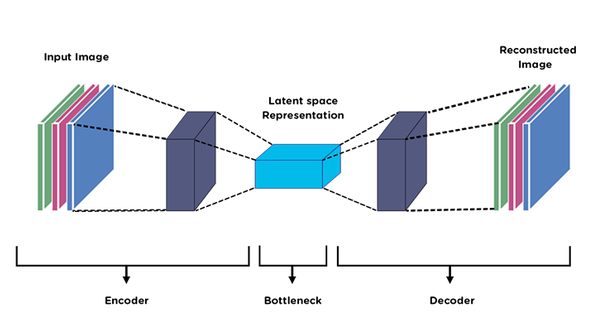
\includegraphics{./figures/autoencoder.png}

The idea for autoencoders was created by the PDP group back in 1986 and
published as \emph{Learning Internal Representations by Error
    Propagation} (Rumelhart et al., 1986). The idea behind them is
conceptually pretty simple. On the surface, an autoencoder is the same
as any other neural network. Inputs are passed through the network
through its layers and optimized via backpropagation. However, the
structure of the autoencoder is one where the inputs are ``squeezed''
through a low-dimensionality middle layer. We call the layers that lead
up to this point the ``encoder'', and the layers that lead away from
this point the ``decoder''.

If we make the output layer the same shape as the input layer, we can
choose an error function that penalizes the difference between the input
and the output. This causes the model to attempt to reconstruct the
input from the output. This is the main idea behind autoencoders: they
are neural networks that attempt to reconstruct their inputs
\emph{through a lower-dimensionality bottleneck}.

After training the model, we can essentially throw away the decoder and
use the encoder as a dimensionality reduction algorithm. In essence, the
encoder becomes a non-linear PCA.

\hypertarget{dataset}{%
    \section{Dataset}\label{dataset}}

To showcase how autoencoders and PCA differ, let's use the MNIST
dataset. This dataset contains 70,000 images of handwritten digits, each
28x28 pixels. The goal is to classify each image as one of the 10
digits.

We specifically use the \texttt{torchvision} version, which contains
more then the \texttt{sklearn} version.

\begin{tcolorbox}[breakable, size=fbox, boxrule=1pt, pad at break*=1mm,colback=cellbackground, colframe=cellborder]
    \prompt{In}{incolor}{2}{\boxspacing}
    \begin{Verbatim}[commandchars=\\\{\}]
        \PY{k+kn}{from} \PY{n+nn}{sklearn}\PY{n+nn}{.}\PY{n+nn}{decomposition} \PY{k+kn}{import} \PY{n}{PCA}
        \PY{k+kn}{from} \PY{n+nn}{torchvision}\PY{n+nn}{.}\PY{n+nn}{datasets} \PY{k+kn}{import} \PY{n}{MNIST}

        \PY{n}{data\PYZus{}dir} \PY{o}{=} \PY{l+s+s1}{\PYZsq{}}\PY{l+s+s1}{../data/raw/}\PY{l+s+s1}{\PYZsq{}}
        \PY{n}{dataset} \PY{o}{=} \PY{n}{MNIST}\PY{p}{(}\PY{n}{data\PYZus{}dir}\PY{p}{,} \PY{n}{train}\PY{o}{=}\PY{k+kc}{True}\PY{p}{,} \PY{n}{download}\PY{o}{=}\PY{k+kc}{True}\PY{p}{)}
    \end{Verbatim}
\end{tcolorbox}

\hypertarget{pca}{%
    \section{PCA}\label{pca}}

With \texttt{scikit-learn}, it's easy to train a PCA model. We simply
need to instantiate a \texttt{PCA} object, and then call \texttt{fit} on
the data. In the background, this does everything we learned in class.

Let's use 2 components, so we can visualize the data in 2D.

\begin{tcolorbox}[breakable, size=fbox, boxrule=1pt, pad at break*=1mm,colback=cellbackground, colframe=cellborder]
    \prompt{In}{incolor}{3}{\boxspacing}
    \begin{Verbatim}[commandchars=\\\{\}]
        \PY{n}{n\PYZus{}components} \PY{o}{=} \PY{l+m+mi}{2}
        \PY{n}{pca} \PY{o}{=} \PY{n}{PCA}\PY{p}{(}\PY{n}{n\PYZus{}components}\PY{o}{=}\PY{n}{n\PYZus{}components}\PY{p}{)}

        \PY{n}{data} \PY{o}{=} \PY{n}{dataset}\PY{o}{.}\PY{n}{data}\PY{o}{.}\PY{n}{numpy}\PY{p}{(}\PY{p}{)}
        \PY{n}{data} \PY{o}{=} \PY{n}{data}\PY{o}{.}\PY{n}{reshape}\PY{p}{(}\PY{o}{\PYZhy{}}\PY{l+m+mi}{1}\PY{p}{,} \PY{l+m+mi}{28} \PY{o}{*} \PY{l+m+mi}{28}\PY{p}{)}  \PY{c+c1}{\PYZsh{} Need to reshape into flattened array for PCA}
        \PY{n}{pca}\PY{o}{.}\PY{n}{fit}\PY{p}{(}\PY{n}{data}\PY{p}{)}
    \end{Verbatim}
\end{tcolorbox}

\begin{tcolorbox}[breakable, size=fbox, boxrule=.5pt, pad at break*=1mm, opacityfill=0]
    \prompt{Out}{outcolor}{3}{\boxspacing}
    \begin{Verbatim}[commandchars=\\\{\}]
        PCA(n\_components=2)
    \end{Verbatim}
\end{tcolorbox}

With the model trained, we can visualize what their principal components
look like.

\begin{tcolorbox}[breakable, size=fbox, boxrule=1pt, pad at break*=1mm,colback=cellbackground, colframe=cellborder]
    \prompt{In}{incolor}{4}{\boxspacing}
    \begin{Verbatim}[commandchars=\\\{\}]
        \PY{n}{test\PYZus{}dataset} \PY{o}{=} \PY{n}{MNIST}\PY{p}{(}\PY{n}{data\PYZus{}dir}\PY{p}{,} \PY{n}{train}\PY{o}{=}\PY{k+kc}{False}\PY{p}{,} \PY{n}{download}\PY{o}{=}\PY{k+kc}{True}\PY{p}{)}
    \end{Verbatim}
\end{tcolorbox}

\begin{tcolorbox}[breakable, size=fbox, boxrule=1pt, pad at break*=1mm,colback=cellbackground, colframe=cellborder]
    \prompt{In}{incolor}{5}{\boxspacing}
    \begin{Verbatim}[commandchars=\\\{\}]
        \PY{k+kn}{import} \PY{n+nn}{seaborn} \PY{k}{as} \PY{n+nn}{sns}
        \PY{n}{pc} \PY{o}{=} \PY{n}{pca}\PY{o}{.}\PY{n}{transform}\PY{p}{(}\PY{n}{test\PYZus{}dataset}\PY{o}{.}\PY{n}{data}\PY{o}{.}\PY{n}{numpy}\PY{p}{(}\PY{p}{)}\PY{o}{.}\PY{n}{reshape}\PY{p}{(}\PY{o}{\PYZhy{}}\PY{l+m+mi}{1}\PY{p}{,} \PY{l+m+mi}{28} \PY{o}{*} \PY{l+m+mi}{28}\PY{p}{)}\PY{p}{)}
        \PY{n}{sns}\PY{o}{.}\PY{n}{scatterplot}\PY{p}{(}\PY{n}{x}\PY{o}{=}\PY{n}{pc}\PY{p}{[}\PY{p}{:}\PY{p}{,} \PY{l+m+mi}{0}\PY{p}{]}\PY{p}{,} \PY{n}{y}\PY{o}{=}\PY{n}{pc}\PY{p}{[}\PY{p}{:}\PY{p}{,} \PY{l+m+mi}{1}\PY{p}{]}\PY{p}{,} \PY{n}{hue}\PY{o}{=}\PY{n}{test\PYZus{}dataset}\PY{o}{.}\PY{n}{targets}\PY{p}{,} \PY{n}{palette}\PY{o}{=}\PY{l+s+s1}{\PYZsq{}}\PY{l+s+s1}{tab10}\PY{l+s+s1}{\PYZsq{}}\PY{p}{)}
    \end{Verbatim}
\end{tcolorbox}

\begin{tcolorbox}[breakable, size=fbox, boxrule=.5pt, pad at break*=1mm, opacityfill=0]
    \prompt{Out}{outcolor}{5}{\boxspacing}
    \begin{Verbatim}[commandchars=\\\{\}]
        <AxesSubplot: >
    \end{Verbatim}
\end{tcolorbox}

\begin{center}
    \adjustimage{max size={0.9\linewidth}{0.9\paperheight}}{report_files/report_16_1.png}
\end{center}
{ \hspace*{\fill} \\}

Not bad! We can generally see each digit lives in its own cluster,
meaning a clustering algorithm should be able to classify the data.
However, we can see that the 2D projection is not perfect. For example,
the 1s and 7s are mixed together, and the 4s and 9s are mixed together.

Let's see if we can do better with an autoencoder.

\hypertarget{autoencoders}{%
    \section{Autoencoders}\label{autoencoders}}

\href{https://pytorch.org/}{PyTorch} is a popular deep learning
framework with a lot of built-in functionality for neural networks. It
allows us to focus on the structure of the network, while it takes care
of things like gradient calculations, backpropagation, and optimization.

\href{https://www.pytorchlightning.ai/}{PyTorch Lightning} is a
framework built on top of PyTorch that automates certain tasks, like
training and validation loops. It also provides a lot of built-in
functionality for common tasks, like logging and checkpointing.

While it's possible to create autoencoders in native PyTorch, we will
use PyTorch Lightning to simplify the logic.

\begin{tcolorbox}[breakable, size=fbox, boxrule=1pt, pad at break*=1mm,colback=cellbackground, colframe=cellborder]
    \prompt{In}{incolor}{6}{\boxspacing}
    \begin{Verbatim}[commandchars=\\\{\}]
        \PY{k+kn}{from} \PY{n+nn}{autoencoder\PYZus{}mnist}\PY{n+nn}{.}\PY{n+nn}{data}\PY{n+nn}{.}\PY{n+nn}{mnist\PYZus{}loader} \PY{k+kn}{import} \PY{n}{MNISTLoader}

        \PY{c+c1}{\PYZsh{} Custom DataLoader that wraps the same MNIST seen earlier }
        \PY{n}{dm} \PY{o}{=} \PY{n}{MNISTLoader}\PY{p}{(}\PY{n}{data\PYZus{}dir}\PY{p}{,} \PY{n}{batch\PYZus{}size}\PY{o}{=}\PY{l+m+mi}{1048}\PY{p}{,} \PY{n}{num\PYZus{}workers}\PY{o}{=}\PY{l+m+mi}{12}\PY{p}{)}
    \end{Verbatim}
\end{tcolorbox}

Now, let's define our model infrastructure. Even with PyTorch Lightning
there's still a bit of boilerplate code, so I've abstracted it away
inside a module. If you're interested in the actual details, you can
check out the \href{https://github.com/nickthegroot/autoencoder-mnist/blob/main/autoencoder_mnist/models/autoencoder_fc.py}{\texttt{autoencoder\_mnist/models/autoencoder\_fc.py}} file

\begin{tcolorbox}[breakable, size=fbox, boxrule=1pt, pad at break*=1mm,colback=cellbackground, colframe=cellborder]
    \prompt{In}{incolor}{7}{\boxspacing}
    \begin{Verbatim}[commandchars=\\\{\}]
        \PY{k+kn}{from} \PY{n+nn}{autoencoder\PYZus{}mnist}\PY{n+nn}{.}\PY{n+nn}{models}\PY{n+nn}{.}\PY{n+nn}{autoencoder\PYZus{}fc} \PY{k+kn}{import} \PY{n}{AutoencoderFC}
        \PY{k+kn}{from} \PY{n+nn}{pytorch\PYZus{}lightning}\PY{n+nn}{.}\PY{n+nn}{utilities}\PY{n+nn}{.}\PY{n+nn}{model\PYZus{}summary} \PY{k+kn}{import} \PY{n}{ModelSummary}

        \PY{n}{n\PYZus{}components} \PY{o}{=} \PY{l+m+mi}{2}
        \PY{n}{model} \PY{o}{=} \PY{n}{AutoencoderFC}\PY{p}{(}\PY{n}{n\PYZus{}components}\PY{p}{,} \PY{l+m+mf}{1e\PYZhy{}3}\PY{p}{)}
        \PY{n}{ModelSummary}\PY{p}{(}\PY{n}{model}\PY{p}{,} \PY{n}{max\PYZus{}depth} \PY{o}{=} \PY{l+m+mi}{1}\PY{p}{)}
    \end{Verbatim}
\end{tcolorbox}

\begin{tcolorbox}[breakable, size=fbox, boxrule=.5pt, pad at break*=1mm, opacityfill=0]
    \prompt{Out}{outcolor}{7}{\boxspacing}
    \begin{Verbatim}[commandchars=\\\{\}]
        | Name    | Type       | Params | In sizes       | Out sizes
        ----------------------------------------------------------------------
        0 | encoder | Sequential | 109 K  | [1, 1, 28, 28] | [1, 2]
        1 | decoder | Sequential | 110 K  | [1, 2]         | [1, 28, 28]
        ----------------------------------------------------------------------
        219 K     Trainable params
        0         Non-trainable params
        219 K     Total params
        0.879     Total estimated model params size (MB)
    \end{Verbatim}
\end{tcolorbox}

We can see two parts to the model: the encoder and decoder. As
explained, the encoder takes the original \((28, 28)\) image and
squeezes it down to a lower \((2)\) dimensionality representation, while
the decoder brings it right back up to a \((28, 28)\) image. Note that
the leading \((1)\) is the batch size.

Let's dig into what each part is actually composed of.

\begin{tcolorbox}[breakable, size=fbox, boxrule=1pt, pad at break*=1mm,colback=cellbackground, colframe=cellborder]
    \prompt{In}{incolor}{8}{\boxspacing}
    \begin{Verbatim}[commandchars=\\\{\}]
        \PY{n}{ModelSummary}\PY{p}{(}\PY{n}{model}\PY{p}{,} \PY{n}{max\PYZus{}depth} \PY{o}{=} \PY{l+m+mi}{2}\PY{p}{)}
    \end{Verbatim}
\end{tcolorbox}

\begin{tcolorbox}[breakable, size=fbox, boxrule=.5pt, pad at break*=1mm, opacityfill=0]
    \prompt{Out}{outcolor}{8}{\boxspacing}
    \begin{Verbatim}[commandchars=\\\{\}]
        | Name      | Type       | Params | In sizes       | Out sizes
        -------------------------------------------------------------------------
        0  | encoder   | Sequential | 109 K  | [1, 1, 28, 28] | [1, 2]
        1  | encoder.0 | Flatten    | 0      | [1, 1, 28, 28] | [1, 784]
        2  | encoder.1 | Linear     | 100 K  | [1, 784]       | [1, 128]
        3  | encoder.2 | ReLU       | 0      | [1, 128]       | [1, 128]
        4  | encoder.3 | Linear     | 8.3 K  | [1, 128]       | [1, 64]
        5  | encoder.4 | ReLU       | 0      | [1, 64]        | [1, 64]
        6  | encoder.5 | Linear     | 780    | [1, 64]        | [1, 12]
        7  | encoder.6 | ReLU       | 0      | [1, 12]        | [1, 12]
        8  | encoder.7 | Linear     | 26     | [1, 12]        | [1, 2]
        9  | decoder   | Sequential | 110 K  | [1, 2]         | [1, 28, 28]
        10 | decoder.0 | Linear     | 36     | [1, 2]         | [1, 12]
        11 | decoder.1 | ReLU       | 0      | [1, 12]        | [1, 12]
        12 | decoder.2 | Linear     | 832    | [1, 12]        | [1, 64]
        13 | decoder.3 | ReLU       | 0      | [1, 64]        | [1, 64]
        14 | decoder.4 | Linear     | 8.3 K  | [1, 64]        | [1, 128]
        15 | decoder.5 | ReLU       | 0      | [1, 128]       | [1, 128]
        16 | decoder.6 | Linear     | 101 K  | [1, 128]       | [1, 784]
        17 | decoder.7 | Sigmoid    | 0      | [1, 784]       | [1, 784]
        18 | decoder.8 | Unflatten  | 0      | [1, 784]       | [1, 28, 28]
        -------------------------------------------------------------------------
        219 K     Trainable params
        0         Non-trainable params
        219 K     Total params
        0.879     Total estimated model params size (MB)
    \end{Verbatim}
\end{tcolorbox}

The encoder is composed of 7 layers. Looking closer, however, we notice
that it's only made up of three trainable layers (\texttt{Linear}). The
\texttt{Flatten} layer ensures our inputs are the correct shape when
passed around the model, while the \texttt{ReLU} is the an activation
function like \texttt{Sigmoid}.

We can also see that the decoder is a mirror image of the encoder. Note
that it doesn't necessarily have to be, but it's a good starting point
and simplifies some of the logic.

The biggest drawback of autoencoders is that they are computationally
expensive (especially compared to PCA). As such, we will load in a model
I previously trained on my desktop with GPU acceleration.

\begin{tcolorbox}[breakable, size=fbox, boxrule=1pt, pad at break*=1mm,colback=cellbackground, colframe=cellborder]
    \prompt{In}{incolor}{9}{\boxspacing}
    \begin{Verbatim}[commandchars=\\\{\}]
        \PY{n}{model} \PY{o}{=} \PY{n}{AutoencoderFC}\PY{o}{.}\PY{n}{load\PYZus{}from\PYZus{}checkpoint}\PY{p}{(}
        \PY{l+s+s1}{\PYZsq{}}\PY{l+s+s1}{../models/20221206\PYZhy{}fc\PYZhy{}2/model.ckpt}\PY{l+s+s1}{\PYZsq{}}\PY{p}{,}
        \PY{n}{n\PYZus{}components}\PY{o}{=}\PY{l+m+mi}{2}\PY{p}{,}
        \PY{n}{lr}\PY{o}{=}\PY{l+m+mf}{1e\PYZhy{}3}\PY{p}{,}
        \PY{p}{)}
    \end{Verbatim}
\end{tcolorbox}

Finally, we can visualize the results. We'll use the \texttt{test} set
to see how well the model generalizes.

\begin{tcolorbox}[breakable, size=fbox, boxrule=1pt, pad at break*=1mm,colback=cellbackground, colframe=cellborder]
    \prompt{In}{incolor}{10}{\boxspacing}
    \begin{Verbatim}[commandchars=\\\{\}]
        \PY{k+kn}{import} \PY{n+nn}{torch}

        \PY{n}{encoder} \PY{o}{=} \PY{n}{model}\PY{o}{.}\PY{n}{encoder}
        \PY{n}{encoder}\PY{o}{.}\PY{n}{eval}\PY{p}{(}\PY{p}{)}
        \PY{n}{dm}\PY{o}{.}\PY{n}{setup}\PY{p}{(}\PY{l+s+s1}{\PYZsq{}}\PY{l+s+s1}{test}\PY{l+s+s1}{\PYZsq{}}\PY{p}{)}

        \PY{n}{representations} \PY{o}{=} \PY{p}{[}\PY{p}{]}
        \PY{n}{targets} \PY{o}{=} \PY{p}{[}\PY{p}{]}
        \PY{k}{with} \PY{n}{torch}\PY{o}{.}\PY{n}{no\PYZus{}grad}\PY{p}{(}\PY{p}{)}\PY{p}{:}
        \PY{k}{for} \PY{n}{img}\PY{p}{,} \PY{n}{target} \PY{o+ow}{in} \PY{n}{dm}\PY{o}{.}\PY{n}{predict\PYZus{}dataloader}\PY{p}{(}\PY{p}{)}\PY{p}{:}
        \PY{n}{rep} \PY{o}{=} \PY{n}{encoder}\PY{p}{(}\PY{n}{img}\PY{p}{)}
        \PY{n}{representations}\PY{o}{.}\PY{n}{append}\PY{p}{(}\PY{n}{rep}\PY{p}{)}
        \PY{n}{targets}\PY{o}{.}\PY{n}{append}\PY{p}{(}\PY{n}{target}\PY{p}{)}
    \end{Verbatim}
\end{tcolorbox}

\begin{tcolorbox}[breakable, size=fbox, boxrule=1pt, pad at break*=1mm,colback=cellbackground, colframe=cellborder]
    \prompt{In}{incolor}{11}{\boxspacing}
    \begin{Verbatim}[commandchars=\\\{\}]
        \PY{n}{X} \PY{o}{=} \PY{n}{torch}\PY{o}{.}\PY{n}{vstack}\PY{p}{(}\PY{n}{representations}\PY{p}{)}
        \PY{n}{y} \PY{o}{=} \PY{n}{torch}\PY{o}{.}\PY{n}{hstack}\PY{p}{(}\PY{n}{targets}\PY{p}{)}

        \PY{n}{ax} \PY{o}{=} \PY{n}{sns}\PY{o}{.}\PY{n}{scatterplot}\PY{p}{(}\PY{n}{x}\PY{o}{=}\PY{n}{X}\PY{p}{[}\PY{p}{:}\PY{p}{,} \PY{l+m+mi}{0}\PY{p}{]}\PY{p}{,} \PY{n}{y}\PY{o}{=}\PY{n}{X}\PY{p}{[}\PY{p}{:}\PY{p}{,} \PY{l+m+mi}{1}\PY{p}{]}\PY{p}{,} \PY{n}{hue}\PY{o}{=}\PY{n}{y}\PY{p}{,} \PY{n}{palette}\PY{o}{=}\PY{l+s+s1}{\PYZsq{}}\PY{l+s+s1}{tab10}\PY{l+s+s1}{\PYZsq{}}\PY{p}{)}
        \PY{n}{ax}\PY{o}{.}\PY{n}{set\PYZus{}title}\PY{p}{(}\PY{l+s+s1}{\PYZsq{}}\PY{l+s+s1}{Autoencoder Components}\PY{l+s+s1}{\PYZsq{}}\PY{p}{)}
        \PY{n}{ax}\PY{o}{.}\PY{n}{set\PYZus{}xlabel}\PY{p}{(}\PY{l+s+s1}{\PYZsq{}}\PY{l+s+s1}{Component 1}\PY{l+s+s1}{\PYZsq{}}\PY{p}{)}
        \PY{n}{ax}\PY{o}{.}\PY{n}{set\PYZus{}ylabel}\PY{p}{(}\PY{l+s+s1}{\PYZsq{}}\PY{l+s+s1}{Component 2}\PY{l+s+s1}{\PYZsq{}}\PY{p}{)}
    \end{Verbatim}
\end{tcolorbox}

\begin{tcolorbox}[breakable, size=fbox, boxrule=.5pt, pad at break*=1mm, opacityfill=0]
    \prompt{Out}{outcolor}{11}{\boxspacing}
    \begin{Verbatim}[commandchars=\\\{\}]
        Text(0, 0.5, 'Component 2')
    \end{Verbatim}
\end{tcolorbox}

\begin{center}
    \adjustimage{max size={0.9\linewidth}{0.9\paperheight}}{report_files/report_32_1.png}
\end{center}
{ \hspace*{\fill} \\}

Wow, that's much clearer then PCA! While there's still some overlap
(especially between the 7s and 9s), the clusters are much more distinct.
A Mixture of Gaussian model would be able to model this especially well.
This is a good sign that the autoencoder is able to capture more of
what's important in the data.

Just for fun, let's see what a 3D projection looks like.

\begin{tcolorbox}[breakable, size=fbox, boxrule=1pt, pad at break*=1mm,colback=cellbackground, colframe=cellborder]
    \prompt{In}{incolor}{12}{\boxspacing}
    \begin{Verbatim}[commandchars=\\\{\}]
        \PY{n}{model} \PY{o}{=} \PY{n}{AutoencoderFC}\PY{o}{.}\PY{n}{load\PYZus{}from\PYZus{}checkpoint}\PY{p}{(}
        \PY{l+s+s1}{\PYZsq{}}\PY{l+s+s1}{../models/20221206\PYZhy{}fc\PYZhy{}3/model.ckpt}\PY{l+s+s1}{\PYZsq{}}\PY{p}{,}
        \PY{n}{n\PYZus{}components}\PY{o}{=}\PY{l+m+mi}{3}\PY{p}{,}
        \PY{n}{lr}\PY{o}{=}\PY{l+m+mf}{1e\PYZhy{}3}\PY{p}{,}
        \PY{p}{)}
    \end{Verbatim}
\end{tcolorbox}

\begin{tcolorbox}[breakable, size=fbox, boxrule=1pt, pad at break*=1mm,colback=cellbackground, colframe=cellborder]
    \prompt{In}{incolor}{13}{\boxspacing}
    \begin{Verbatim}[commandchars=\\\{\}]
        \PY{n}{encoder} \PY{o}{=} \PY{n}{model}\PY{o}{.}\PY{n}{encoder}
        \PY{n}{encoder}\PY{o}{.}\PY{n}{eval}\PY{p}{(}\PY{p}{)}

        \PY{n}{representations} \PY{o}{=} \PY{p}{[}\PY{p}{]}
        \PY{n}{targets} \PY{o}{=} \PY{p}{[}\PY{p}{]}
        \PY{k}{with} \PY{n}{torch}\PY{o}{.}\PY{n}{no\PYZus{}grad}\PY{p}{(}\PY{p}{)}\PY{p}{:}
        \PY{k}{for} \PY{n}{img}\PY{p}{,} \PY{n}{target} \PY{o+ow}{in} \PY{n}{dm}\PY{o}{.}\PY{n}{predict\PYZus{}dataloader}\PY{p}{(}\PY{p}{)}\PY{p}{:}
        \PY{n}{rep} \PY{o}{=} \PY{n}{encoder}\PY{p}{(}\PY{n}{img}\PY{p}{)}
        \PY{n}{representations}\PY{o}{.}\PY{n}{append}\PY{p}{(}\PY{n}{rep}\PY{p}{)}
        \PY{n}{targets}\PY{o}{.}\PY{n}{append}\PY{p}{(}\PY{n}{target}\PY{p}{)}
    \end{Verbatim}
\end{tcolorbox}

\begin{tcolorbox}[breakable, size=fbox, boxrule=1pt, pad at break*=1mm,colback=cellbackground, colframe=cellborder]
    \prompt{In}{incolor}{14}{\boxspacing}
    \begin{Verbatim}[commandchars=\\\{\}]
        \PY{k+kn}{import} \PY{n+nn}{matplotlib}\PY{n+nn}{.}\PY{n+nn}{pyplot} \PY{k}{as} \PY{n+nn}{plt}

        \PY{n}{X} \PY{o}{=} \PY{n}{torch}\PY{o}{.}\PY{n}{vstack}\PY{p}{(}\PY{n}{representations}\PY{p}{)}
        \PY{n}{y} \PY{o}{=} \PY{n}{torch}\PY{o}{.}\PY{n}{hstack}\PY{p}{(}\PY{n}{targets}\PY{p}{)}

        \PY{n}{fig} \PY{o}{=} \PY{n}{plt}\PY{o}{.}\PY{n}{figure}\PY{p}{(}\PY{p}{)}
        \PY{n}{ax} \PY{o}{=} \PY{n}{fig}\PY{o}{.}\PY{n}{add\PYZus{}subplot}\PY{p}{(}\PY{n}{projection}\PY{o}{=}\PY{l+s+s1}{\PYZsq{}}\PY{l+s+s1}{3d}\PY{l+s+s1}{\PYZsq{}}\PY{p}{)}

        \PY{n}{ax}\PY{o}{.}\PY{n}{scatter}\PY{p}{(}\PY{n}{X}\PY{p}{[}\PY{p}{:}\PY{p}{,} \PY{l+m+mi}{0}\PY{p}{]}\PY{p}{,} \PY{n}{X}\PY{p}{[}\PY{p}{:}\PY{p}{,} \PY{l+m+mi}{1}\PY{p}{]}\PY{p}{,} \PY{n}{X}\PY{p}{[}\PY{p}{:}\PY{p}{,} \PY{l+m+mi}{2}\PY{p}{]}\PY{p}{,} \PY{n}{c}\PY{o}{=}\PY{n}{y}\PY{p}{,} \PY{n}{cmap}\PY{o}{=}\PY{l+s+s1}{\PYZsq{}}\PY{l+s+s1}{tab10}\PY{l+s+s1}{\PYZsq{}}\PY{p}{)}
    \end{Verbatim}
\end{tcolorbox}

\begin{tcolorbox}[breakable, size=fbox, boxrule=.5pt, pad at break*=1mm, opacityfill=0]
    \prompt{Out}{outcolor}{14}{\boxspacing}
    \begin{Verbatim}[commandchars=\\\{\}]
        <mpl\_toolkits.mplot3d.art3d.Path3DCollection at 0x7f5fd0b8fe80>
    \end{Verbatim}
\end{tcolorbox}

\begin{center}
    \adjustimage{max size={0.9\linewidth}{0.9\paperheight}}{report_files/report_37_1.png}
\end{center}
{ \hspace*{\fill} \\}

While it's harder to visualize, we can see that the clusters are even
more distinct. This is a good sign that the autoencoder is able to
capture more of what's important in the data.

One potential problem with this is that the model itself is pretty
large. Even throwing away the decoder, all the parameters still take up
\textasciitilde{}0.4 MB. This is due to the model requiring a connection
between every layer.

Can't we do anything about that?

\hypertarget{autoencoders-convolutional-neural-networks}{%
    \section{Autoencoders \& Convolutional Neural
      Networks}\label{autoencoders-convolutional-neural-networks}}

Recall that the actual implementation of the encoder/decoder aren't
strict. We can use any layers we want, as long as the output of the
encoder is the same shape as the input of the decoder (and practically,
that the data goes through some dimensionality bottleneck).

Enter: Convolutional Neural Networks.

These are neural networks that are specifically designed to take
advantage of the spatial information within images.

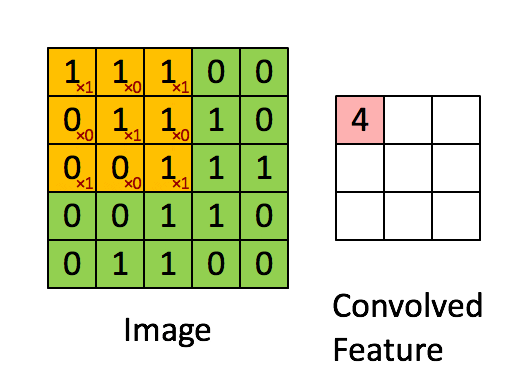
\includegraphics{./figures/cnn.png}

The underlying assumption is that nearby pixels are more likely to be
related than distant pixels. Convolutional neural networks take
advantage of this by creating a sliding window to apply a filter to the
image. This filter is called a \textbf{kernel}, and is essentially a
small matrix that is applied to the image. The kernel is then shifted
over, and the process is repeated. This is called a
\textbf{convolution}.

In the image: - \textbf{The green matrix} represents an image -
\textbf{The yellow matrix} represents a kernel - \textbf{The pink
    matrix} represents the output of the convolution

Let's check out what one of these models would look like in the context
of an autoencoder.

\begin{tcolorbox}[breakable, size=fbox, boxrule=1pt, pad at break*=1mm,colback=cellbackground, colframe=cellborder]
    \prompt{In}{incolor}{15}{\boxspacing}
    \begin{Verbatim}[commandchars=\\\{\}]
        \PY{k+kn}{from} \PY{n+nn}{autoencoder\PYZus{}mnist}\PY{n+nn}{.}\PY{n+nn}{models}\PY{n+nn}{.}\PY{n+nn}{autoencoder\PYZus{}cnn} \PY{k+kn}{import} \PY{n}{AutoencoderCNN}

        \PY{n}{n\PYZus{}components} \PY{o}{=} \PY{l+m+mi}{2}
        \PY{n}{model} \PY{o}{=} \PY{n}{AutoencoderCNN}\PY{p}{(}\PY{n}{n\PYZus{}components}\PY{p}{,} \PY{l+m+mf}{1e\PYZhy{}3}\PY{p}{)}
        \PY{n}{ModelSummary}\PY{p}{(}\PY{n}{model}\PY{p}{,} \PY{n}{max\PYZus{}depth} \PY{o}{=} \PY{l+m+mi}{1}\PY{p}{)}
    \end{Verbatim}
\end{tcolorbox}

\begin{tcolorbox}[breakable, size=fbox, boxrule=.5pt, pad at break*=1mm, opacityfill=0]
    \prompt{Out}{outcolor}{15}{\boxspacing}
    \begin{Verbatim}[commandchars=\\\{\}]
        | Name    | Type       | Params | In sizes       | Out sizes
        -------------------------------------------------------------------------
        0 | encoder | Sequential | 1.4 K  | [1, 1, 28, 28] | [1, 2]
        1 | decoder | Sequential | 4.5 K  | [1, 2]         | [1, 1, 28, 28]
        -------------------------------------------------------------------------
        5.9 K     Trainable params
        0         Non-trainable params
        5.9 K     Total params
        0.024     Total estimated model params size (MB)
    \end{Verbatim}
\end{tcolorbox}

Despite having the same top-level structure, we've cut down on the model
size by almost 50x! This is because the convolutional layers are able to
share parameters across the image through their learned kernels.

\begin{tcolorbox}[breakable, size=fbox, boxrule=1pt, pad at break*=1mm,colback=cellbackground, colframe=cellborder]
    \prompt{In}{incolor}{16}{\boxspacing}
    \begin{Verbatim}[commandchars=\\\{\}]
        \PY{n}{ModelSummary}\PY{p}{(}\PY{n}{model}\PY{p}{,} \PY{n}{max\PYZus{}depth} \PY{o}{=} \PY{l+m+mi}{2}\PY{p}{)}
    \end{Verbatim}
\end{tcolorbox}

\begin{tcolorbox}[breakable, size=fbox, boxrule=.5pt, pad at break*=1mm, opacityfill=0]
    \prompt{Out}{outcolor}{16}{\boxspacing}
    \begin{Verbatim}[commandchars=\\\{\}]
        | Name      | Type            | Params | In sizes        | Out sizes
        --------------------------------------------------------------------------------
        ---
        0  | encoder   | Sequential      | 1.4 K  | [1, 1, 28, 28]  | [1, 2]
        1  | encoder.0 | Conv2d          | 160    | [1, 1, 28, 28]  | [1, 16, 10, 10]
        2  | encoder.1 | ReLU            | 0      | [1, 16, 10, 10] | [1, 16, 10, 10]
        3  | encoder.2 | MaxPool2d       | 0      | [1, 16, 10, 10] | [1, 16, 5, 5]
        4  | encoder.3 | Conv2d          | 1.2 K  | [1, 16, 5, 5]   | [1, 8, 3, 3]
        5  | encoder.4 | ReLU            | 0      | [1, 8, 3, 3]    | [1, 8, 3, 3]
        6  | encoder.5 | MaxPool2d       | 0      | [1, 8, 3, 3]    | [1, 8, 2, 2]
        7  | encoder.6 | Flatten         | 0      | [1, 8, 2, 2]    | [1, 32]
        8  | encoder.7 | Linear          | 66     | [1, 32]         | [1, 2]
        9  | decoder   | Sequential      | 4.5 K  | [1, 2]          | [1, 1, 28, 28]
        10 | decoder.0 | Linear          | 96     | [1, 2]          | [1, 32]
        11 | decoder.1 | Unflatten       | 0      | [1, 32]         | [1, 8, 2, 2]
        12 | decoder.2 | ConvTranspose2d | 1.2 K  | [1, 8, 2, 2]    | [1, 16, 5, 5]
        13 | decoder.3 | ReLU            | 0      | [1, 16, 5, 5]   | [1, 16, 5, 5]
        14 | decoder.4 | ConvTranspose2d | 3.2 K  | [1, 16, 5, 5]   | [1, 8, 15, 15]
        15 | decoder.5 | ReLU            | 0      | [1, 8, 15, 15]  | [1, 8, 15, 15]
        16 | decoder.6 | ConvTranspose2d | 33     | [1, 8, 15, 15]  | [1, 1, 28, 28]
        17 | decoder.7 | Sigmoid         | 0      | [1, 1, 28, 28]  | [1, 1, 28, 28]
        --------------------------------------------------------------------------------
        ---
        5.9 K     Trainable params
        0         Non-trainable params
        5.9 K     Total params
        0.024     Total estimated model params size (MB)
    \end{Verbatim}
\end{tcolorbox}

The encoder is composed of 9 layers. Much like the fully-connected
model, we notice that it's only made up of three trainable
\texttt{Conv2d} layers and one trainable \texttt{Linear} layer. The
\texttt{Flatten} and \texttt{ReLU} layers work the same way as in the
fully-connected model.

The \texttt{MaxPool2d} function as a way of downsampling the spatial
information of the image. Recall that kernels only really look at the
nearby pixels and miss out on the larger picture. \texttt{MaxPool2d}
serves to aggregate this information in larger and larger chunks as we
go down the model. This is called \textbf{pooling}.

Let's see how this model performs. Once again, we'll use a model I
previously trained on my desktop with GPU acceleration.

\begin{tcolorbox}[breakable, size=fbox, boxrule=1pt, pad at break*=1mm,colback=cellbackground, colframe=cellborder]
    \prompt{In}{incolor}{17}{\boxspacing}
    \begin{Verbatim}[commandchars=\\\{\}]
        \PY{n}{model} \PY{o}{=} \PY{n}{AutoencoderCNN}\PY{o}{.}\PY{n}{load\PYZus{}from\PYZus{}checkpoint}\PY{p}{(}
        \PY{l+s+s1}{\PYZsq{}}\PY{l+s+s1}{../models/20221206\PYZhy{}cnn\PYZhy{}2/model.ckpt}\PY{l+s+s1}{\PYZsq{}}\PY{p}{,}
        \PY{n}{n\PYZus{}components}\PY{o}{=}\PY{l+m+mi}{2}\PY{p}{,}
        \PY{n}{lr}\PY{o}{=}\PY{l+m+mf}{1e\PYZhy{}3}\PY{p}{,}
        \PY{p}{)}
    \end{Verbatim}
\end{tcolorbox}

\begin{tcolorbox}[breakable, size=fbox, boxrule=1pt, pad at break*=1mm,colback=cellbackground, colframe=cellborder]
    \prompt{In}{incolor}{18}{\boxspacing}
    \begin{Verbatim}[commandchars=\\\{\}]
        \PY{n}{encoder} \PY{o}{=} \PY{n}{model}\PY{o}{.}\PY{n}{encoder}
        \PY{n}{encoder}\PY{o}{.}\PY{n}{eval}\PY{p}{(}\PY{p}{)}

        \PY{n}{representations} \PY{o}{=} \PY{p}{[}\PY{p}{]}
        \PY{n}{targets} \PY{o}{=} \PY{p}{[}\PY{p}{]}
        \PY{k}{with} \PY{n}{torch}\PY{o}{.}\PY{n}{no\PYZus{}grad}\PY{p}{(}\PY{p}{)}\PY{p}{:}
        \PY{k}{for} \PY{n}{img}\PY{p}{,} \PY{n}{target} \PY{o+ow}{in} \PY{n}{dm}\PY{o}{.}\PY{n}{predict\PYZus{}dataloader}\PY{p}{(}\PY{p}{)}\PY{p}{:}
        \PY{n}{rep} \PY{o}{=} \PY{n}{encoder}\PY{p}{(}\PY{n}{img}\PY{p}{)}
        \PY{n}{representations}\PY{o}{.}\PY{n}{append}\PY{p}{(}\PY{n}{rep}\PY{p}{)}
        \PY{n}{targets}\PY{o}{.}\PY{n}{append}\PY{p}{(}\PY{n}{target}\PY{p}{)}
    \end{Verbatim}
\end{tcolorbox}

\begin{tcolorbox}[breakable, size=fbox, boxrule=1pt, pad at break*=1mm,colback=cellbackground, colframe=cellborder]
    \prompt{In}{incolor}{19}{\boxspacing}
    \begin{Verbatim}[commandchars=\\\{\}]
        \PY{n}{X} \PY{o}{=} \PY{n}{torch}\PY{o}{.}\PY{n}{vstack}\PY{p}{(}\PY{n}{representations}\PY{p}{)}
        \PY{n}{y} \PY{o}{=} \PY{n}{torch}\PY{o}{.}\PY{n}{hstack}\PY{p}{(}\PY{n}{targets}\PY{p}{)}

        \PY{n}{ax} \PY{o}{=} \PY{n}{sns}\PY{o}{.}\PY{n}{scatterplot}\PY{p}{(}\PY{n}{x}\PY{o}{=}\PY{n}{X}\PY{p}{[}\PY{p}{:}\PY{p}{,} \PY{l+m+mi}{0}\PY{p}{]}\PY{p}{,} \PY{n}{y}\PY{o}{=}\PY{n}{X}\PY{p}{[}\PY{p}{:}\PY{p}{,} \PY{l+m+mi}{1}\PY{p}{]}\PY{p}{,} \PY{n}{hue}\PY{o}{=}\PY{n}{y}\PY{p}{,} \PY{n}{palette}\PY{o}{=}\PY{l+s+s1}{\PYZsq{}}\PY{l+s+s1}{tab10}\PY{l+s+s1}{\PYZsq{}}\PY{p}{)}
        \PY{n}{ax}\PY{o}{.}\PY{n}{set\PYZus{}title}\PY{p}{(}\PY{l+s+s1}{\PYZsq{}}\PY{l+s+s1}{Autoencoder Components}\PY{l+s+s1}{\PYZsq{}}\PY{p}{)}
        \PY{n}{ax}\PY{o}{.}\PY{n}{set\PYZus{}xlabel}\PY{p}{(}\PY{l+s+s1}{\PYZsq{}}\PY{l+s+s1}{Component 1}\PY{l+s+s1}{\PYZsq{}}\PY{p}{)}
        \PY{n}{ax}\PY{o}{.}\PY{n}{set\PYZus{}ylabel}\PY{p}{(}\PY{l+s+s1}{\PYZsq{}}\PY{l+s+s1}{Component 2}\PY{l+s+s1}{\PYZsq{}}\PY{p}{)}
    \end{Verbatim}
\end{tcolorbox}

\begin{tcolorbox}[breakable, size=fbox, boxrule=.5pt, pad at break*=1mm, opacityfill=0]
    \prompt{Out}{outcolor}{19}{\boxspacing}
    \begin{Verbatim}[commandchars=\\\{\}]
        Text(0, 0.5, 'Component 2')
    \end{Verbatim}
\end{tcolorbox}

\begin{center}
    \adjustimage{max size={0.9\linewidth}{0.9\paperheight}}{report_files/report_52_1.png}
\end{center}
{ \hspace*{\fill} \\}

While this certainly isn't as good as the fully-connected model, it
still manages to get the general idea across (and at 50x less the size)!

\hypertarget{conclusion}{%
    \section{Conclusion}\label{conclusion}}

I learned a lot over the course of this project. While I had briefly
heard of autoencoders in another course, I never really understood what
they were or how they worked.

When this course started talking about PCA, I realized that autoencoders
were essentially a more complex version of PCA. That gave me the idea to
try and implement one myself and really dig into how they work / what
they're capable of. To that end, I believe this project has done its job
many times over. I'm leaving this course with a much better
understanding of the strengths and weaknesses of PCA and autoencoders.

Given more time, I would love to expand my research into how different
encoder/decoders affect the performance of the model. For example, how
asymmetric encoder/decoder structures affect the performance of the
model. When researching, some sources mentioned that asymmetric
encoder/decoder structures are better at certain tasks, and I would love
to see if/when that's true.

I would also love to explore how autoencoders are used as a piece of
more complex models, such as Stable Diffusion (the image-generating AI
taking the internet by storm). The ability to take a high-dimensional
input and compress it into a low-dimensional latent representation is a
powerful tool, and I'm sure more powerful/complex models have been built
on top of it.


% Add a bibliography block to the postdoc



\end{document}
